\documentclass{article}

\usepackage{graphicx}
\usepackage{tikz}
\usepackage{tikzsymbols}
\usetikzlibrary{calc,patterns,shapes.geometric}
\pagestyle{empty}
\usepackage[margin=0pt]{geometry}
\geometry{papersize={14in,12in}}

\def\centerarc[#1](#2)(#3:#4:#5){\draw[#1] ($(#2)+({#5*cos(#3)},{#5*sin(#3)})$) arc (#3:#4:#5);}

\begin{document}
	\begin{figure}
		\centering
		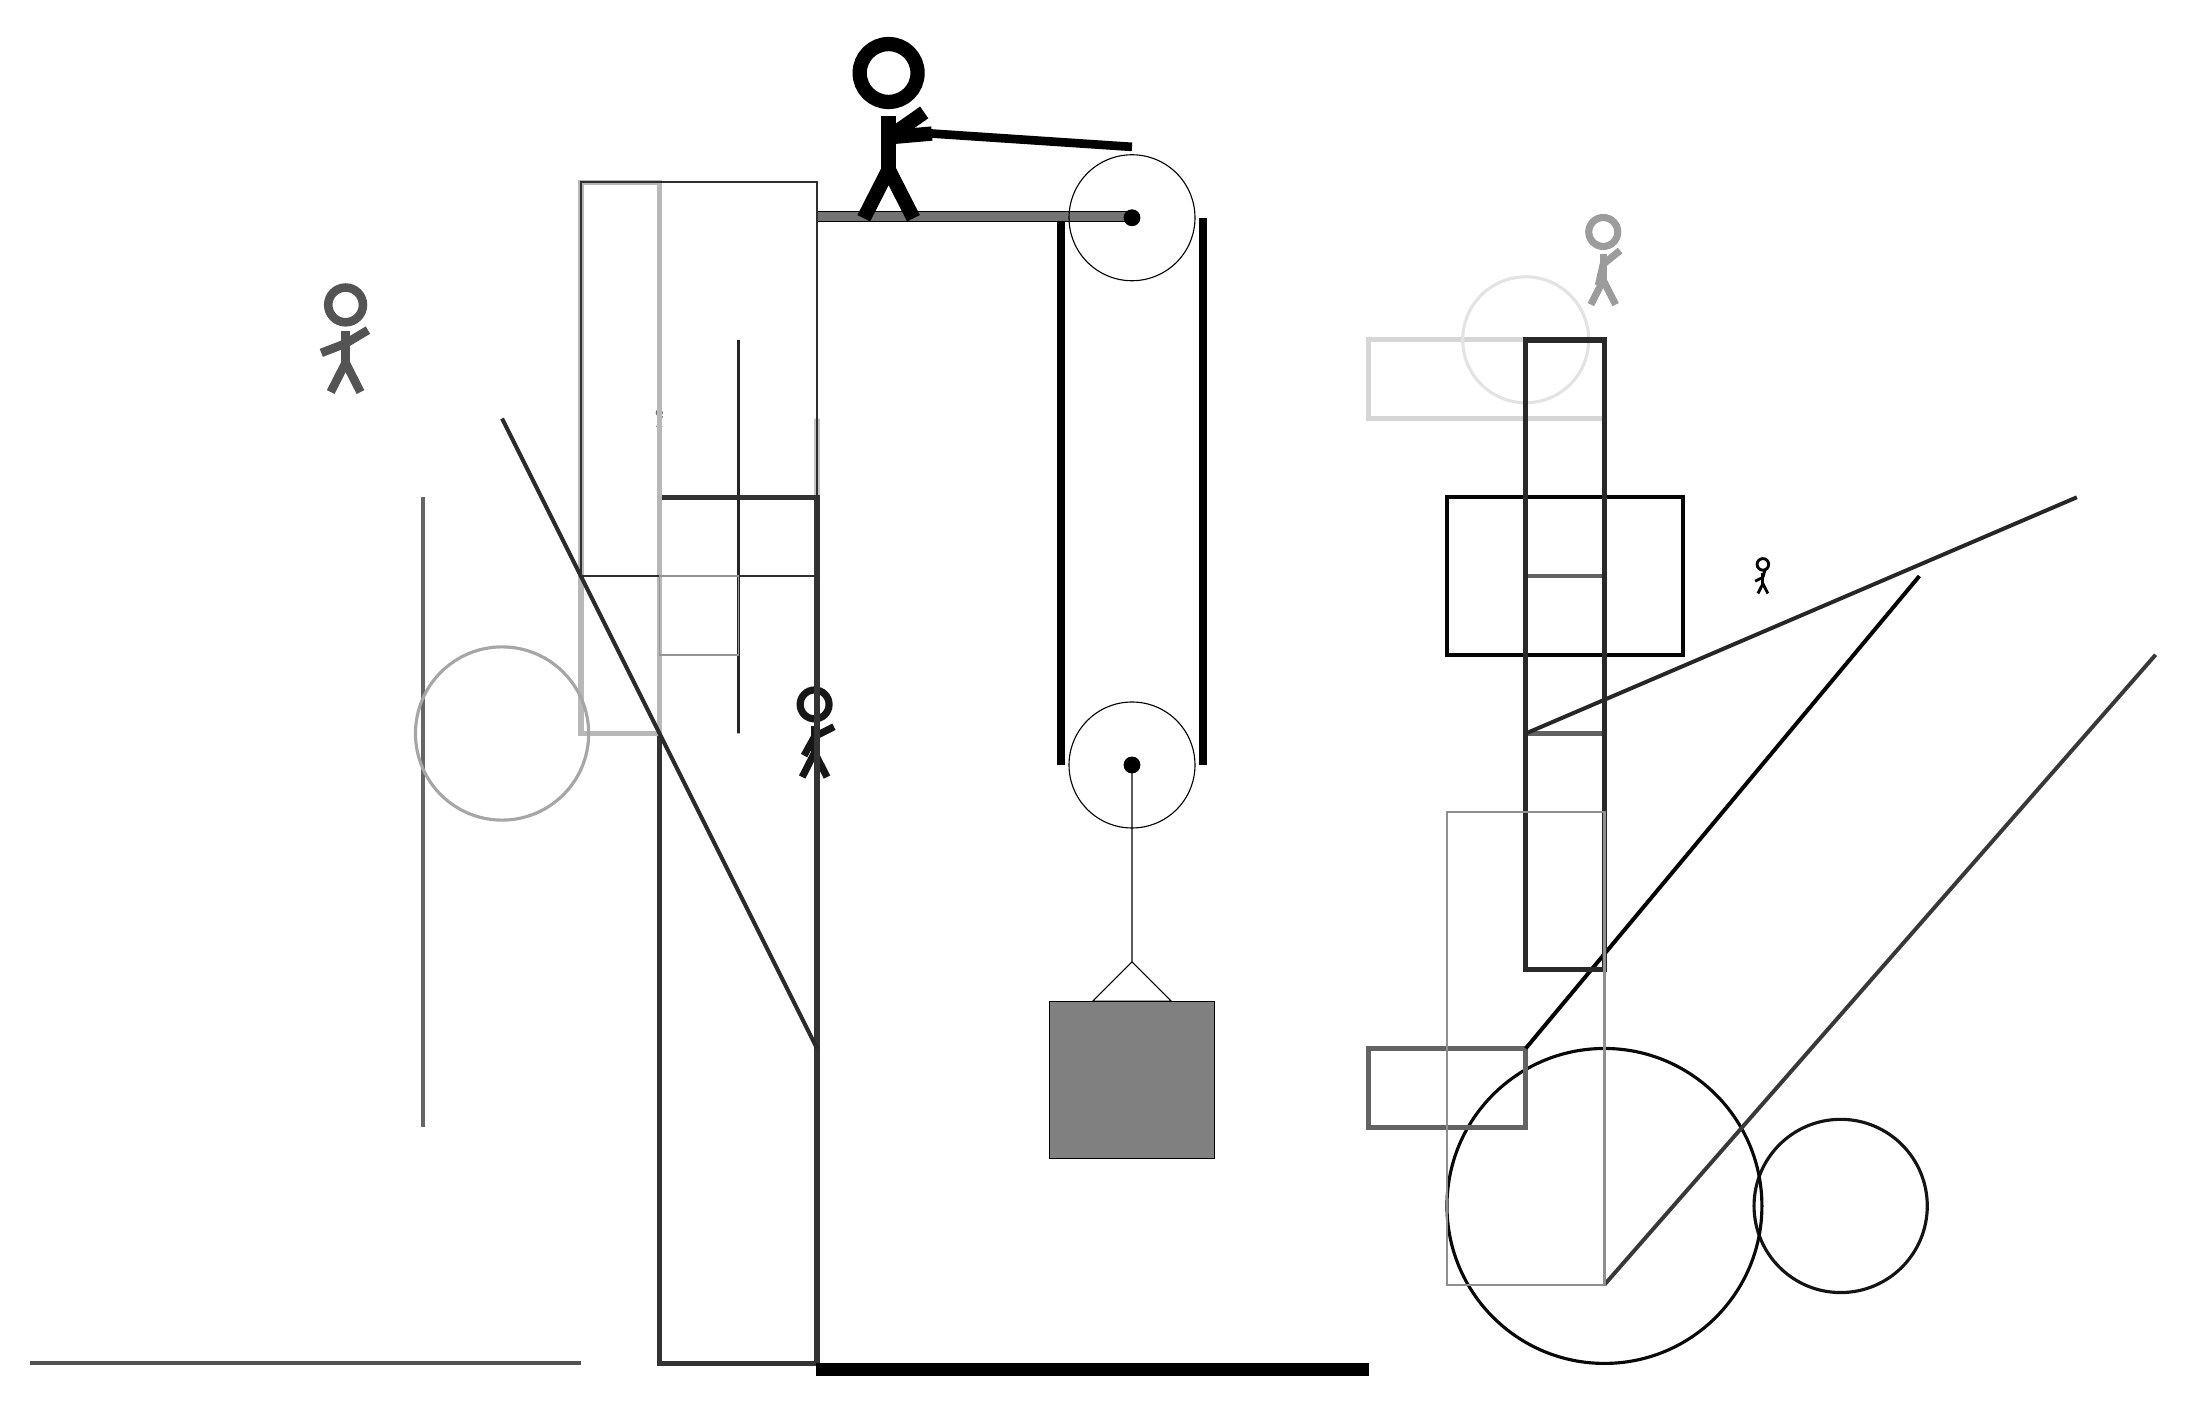
\begin{tikzpicture}
			%%%%% START %%%%%
			
			\draw[fill=black!55] (-2, 11.5) rectangle (2, 11.625);
			
			\draw (2, 4.6) circle (0.8);
			\draw[fill=black] (2, 4.6) circle (0.1);
			
			\draw (2, 11.55) circle (0.8);
			\draw[fill=black] (2, 11.55) circle (0.1);
			
			\draw (2, 4.6) -- (2, 2.1) -- (1.5, 1.6) -- (2.5, 1.6) -- (2, 2.1);
			\draw[fill=black!50] (0.95, 1.6) rectangle (3.05, -0.4);
			
			\draw[line width=1.1mm] (1.1, 11.5) -- (1.1, 4.6);
			\centerarc[line width=1.1mm](2, 4.6)(180:360:0.9);
			\draw[line width=1.1mm](2.9, 4.6) -- (2.9, 11.55);
			\centerarc[line width=1.1mm](2, 11.55)(0:90:0.9);
			\draw[line width=1.1mm](2, 12.45) -- (-1, 12.65);
			
			\draw [line width=0.4mm, color=black!92](11, -1) circle (1.1);
			
			\draw[line width=0.6mm, color=black!16] (5, 10) rectangle (8, 9);
			\draw[line width=0.6mm, color=black!62] (7, 7) rectangle (8, 5);
			\draw[line width=0.4mm, color=black!86] (-3, 5) rectangle (-3, 10);
			\draw [line width=0.5mm, color=black!86](-3, 7) circle (0.0);
			\node[line width=0.4mm, color=black!39] at (8, 11) {\Strichmaxerl[5][77][39]};
			\node[line width=0.7mm, color=black!67] at (-8, 10) {\Strichmaxerl[6][21][31]};
			\draw[line width=0.5mm, color=black!68](-5, -3) -- (-12, -3);
			\draw [line width=0.4mm, color=black!11](7, 10) circle (0.8);
			\node[line width=0.4mm, color=black!57] at (-4, 9) {\Strichmaxerl[1][83][37]};
			
			\node[line width=0.2mm, color=black!91] at (-2, 5) {\Strichmaxerl[5][61][27]};
			
			\draw [line width=0.4mm, color=black!97](8, -1) circle (2.0);
			\draw[line width=0.5mm, color=black!98] (6, 8) rectangle (9, 6);
			
			\draw[line width=0.6mm, color=black!61] (7, 1) rectangle (5, 0);
			\draw[line width=0.5mm, color=black!99](7, 1) -- (12, 7);
			\draw[line width=0.7mm, color=black!23] (-2, 9) rectangle (-2, 1);
			
			\draw[line width=0.5mm, color=black!60](-7, 8) -- (-7, 0);
			\draw[line width=0.5mm, color=black!78](8, -2) -- (15, 6);
			\draw[line width=0.7mm, color=black!80] (-4, -3) rectangle (-2, 8);
			
			\draw[line width=0.5mm, color=black!85](7, 5) -- (14, 8);
			\draw[line width=0.7mm, color=black!84] (7, 2) rectangle (8, 10);
			\draw[line width=0.7mm, color=black!28] (-4, 12) rectangle (-5, 5);
			\draw[line width=0.5mm, color=black!83](-6, 9) -- (-2, 1);
			\draw [line width=0.4mm, color=black!35](-6, 5) circle (1.1);
			\node[line width=0.3mm, color=black!99] at (10, 7) {\Strichmaxerl[2][27][74]};
			
			\draw[line width=0.3mm, color=black!44] (6, 4) rectangle (8, -2);
			
			\draw[line width=0.3mm, color=black!82] (-2, 12) rectangle (-5, 7);
			\draw[line width=0.2mm, color=black!42] (-3, 6) rectangle (-4, 7);
			
			\node at (-1, 12.65) {\Strichmaxerl[10][-175][35]};
			
			\draw[fill=black] (-2, -3) rectangle (5, -3.15);
			
			%%%%% END %%%%%
		\end{tikzpicture}
	\end{figure}	
\end{document}